\appendix


\section{Methods} % (fold)

\subsection{Muscle naming} % (fold)
\label{ap:sub:muscle_naming}

The abbreviations of the muscles are annotated by F for flexor, E for extensor and B for bi-directional. The numbers (e.g. ED45) mean that this muscle extends those fingers that are denoted by these numbers. Fingers are counted in a way that the thumb is finger 1.

% muscle table vega
\begin{table}[ht]
 	\centering
	\small
 	\begin{tabular}{cll}
		\toprule
			channel \# & muscle & abbr. \\
			\toprule
			\multicolumn{3}{c}{Subject V} \\
			1  &	extensor digitorum communis &	EDC E\\
			2  &  	abductor pollicis longus 	&	APL-E\\
			3  &	extensor carpi ulnaris 		&	ECU-E\\
			4  &	flexor carpi radialis 		&	FCR-F\\
			5  &	abductor pollicis longus 	&	APL-E\\
			6  &	extensor digitorum 4, 5 	&	ED45-E\\
			7  &	extensor digitorum 2, 3 	&	ED23-E\\
			8  &	extensor carpi ulnaris 		&	ECU-E\\
			9  &	brachioradialis 			&	BR-B\\
			10 & 	palmaris longus 			&	PL-F\\
			11 & 	flexor carpi radialis 		&	FCR-F\\
			
			\midrule
			\multicolumn{3}{c}{Subject D}  \\
			1  &	extensor carpi ulnaris          &	ECU-E\\
			2  &  	extensor digitorum 4, 5	        &	ED45-E\\
			3  &	extensor digitorum communis     &	EDC-E\\
			4  &	abductor pollicis longus 	    &	APL-E\\
			5  &	extensor carpi radialis 	    &	ECR-E\\
			6  &	extensor digitorum 2, 3         &	ED23-E\\
			7  &	biceps	                        &	BIC-F\\
			8  &	biceps 		                    &	BIC-F\\
			9  &	flexor digitorum superficialis 	&	FDS-F\\
			10 & 	palmaris longus 		        &	PL-F\\ 
			11 & 	flexor carpi ulnaris 		    &	FCU-F\\
			12 &	flexor carpi radialis 		    &	FCR-F\\
			13 & 	flexor pronator teres		    &	PT-F\\
			14 & 	flexor digitorum profundis 	    &	FDP-F\\
			15 &	triceps 			            &	TRIC-E\\
			16 & 	biceps 			                &	BIC-F\\

			\midrule
			\multicolumn{3}{c}{Subject C} \\
			1  &	flexor carpi ulnaris            &	FCU-F\\
			2  &  	flexor digitorum superficialis	&	FDS-F\\
			3  &	palmaris longus                 &	PL-F\\ 
			4  &	flexor carpi radialis 	        &	FCR-F\\
			5  &	flexor pronator teres 	        &	PT-F\\
			6  &	flexor digitorum profundis      &	FDP-F\\
			7  &	palmaris longus 	            &	PL-F\\
			8  &	biceps 		                    &	BIC-F\\
			9  &	extensor carpi ulnaris		    &	ECU-E\\
			10 & 	extensor digitorum communis 	&	EDC-E\\
			11 & 	extensor digitorum 4, 5			&	ED45-E\\
			12 &	extensor carpi radialis 		&	ECR-E\\
			13 & 	extensor digitorum 2, 3 		&	ED23-E\\
			14 & 	abductor pollicis longus		&	APL-E\\
			15 &	extensor carpi radialis 		&	ECR-E\\
			16 & 	triceps 			            &	TRIC-E\\
		\bottomrule
 	\end{tabular}
 	\caption{Muscle names and functions}
 	\label{app:tab:muscle_naming}
\end{table}
% subsection muscle_naming (end)
% section methods (end)

\section{Results} % (fold)
\label{sg:sec:results}
\begin{figure}[ht]
    \centering
        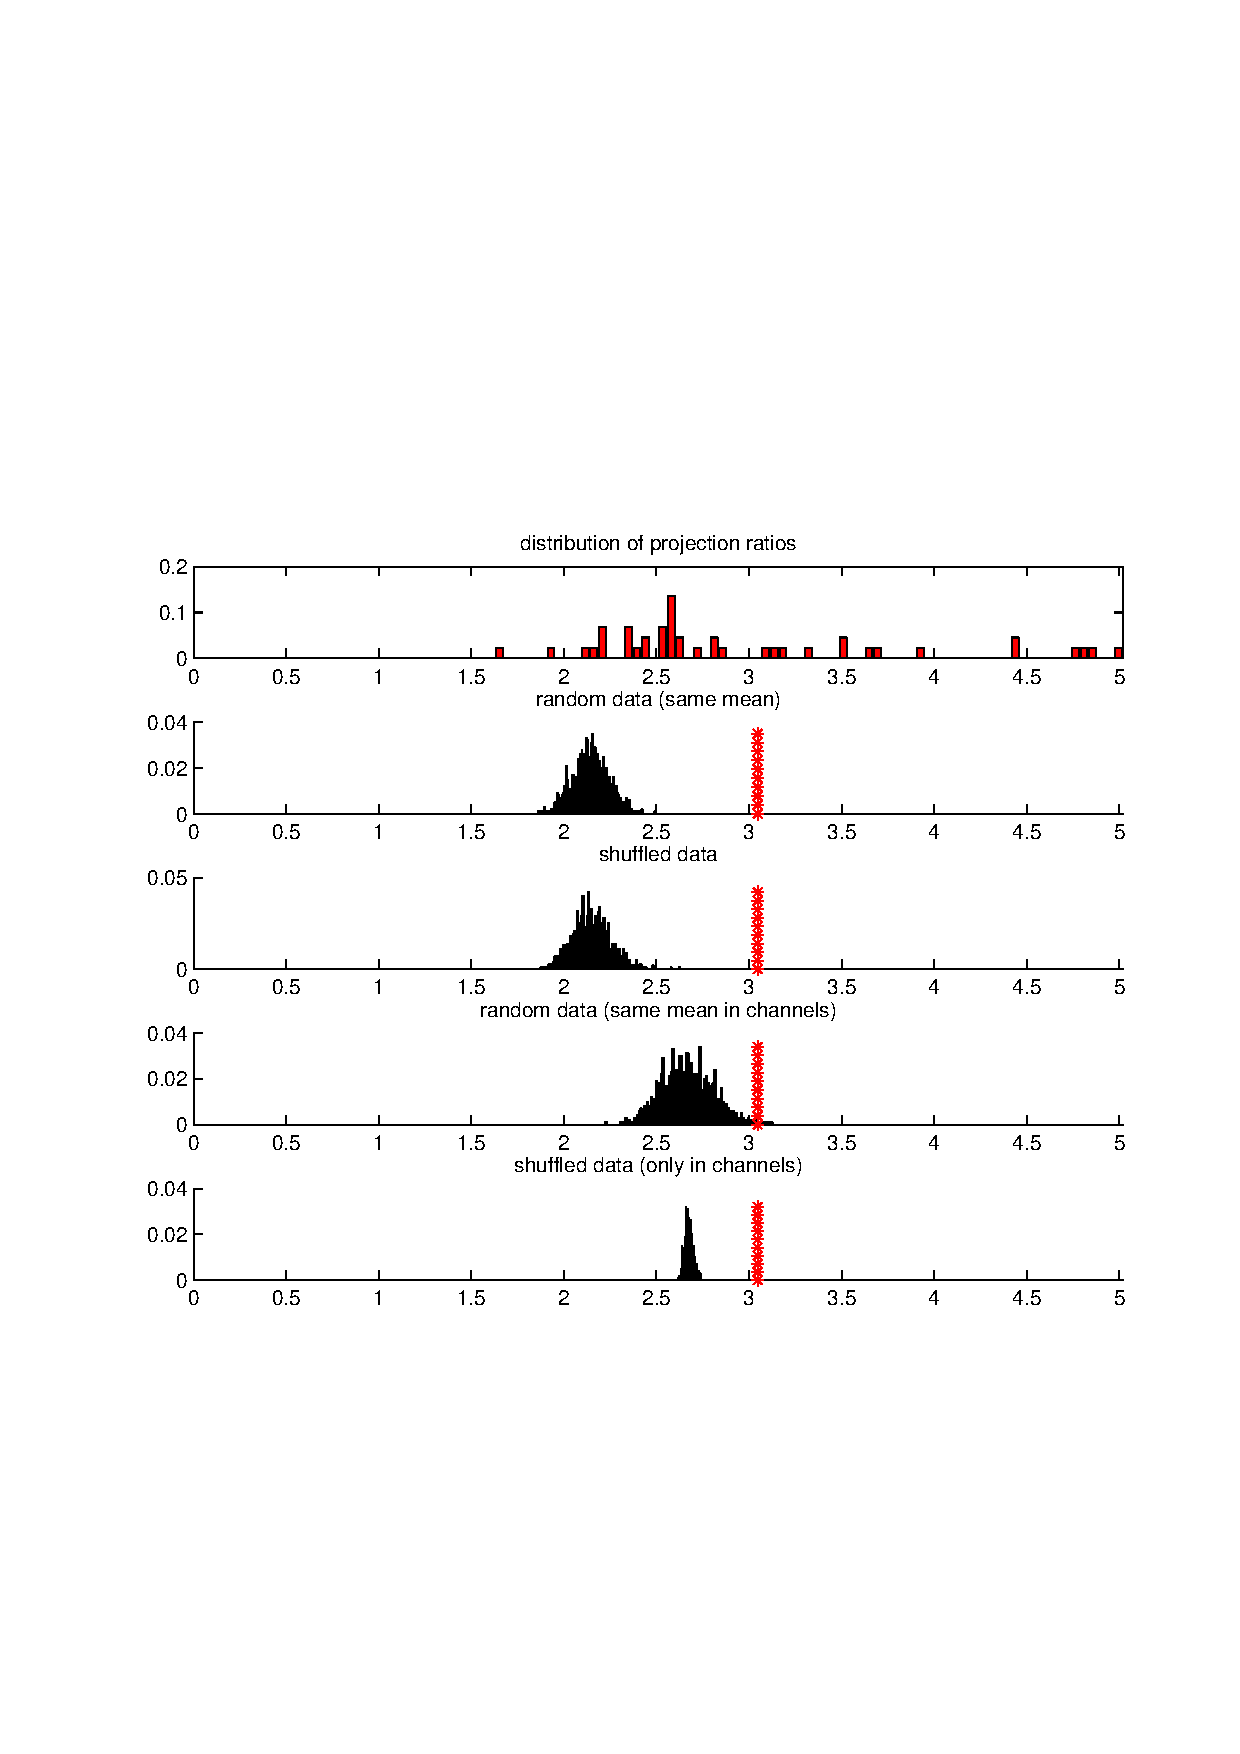
\includegraphics[width=0.8\textwidth]{images/projection_larger0_chalva.pdf}
    \caption{subject C, projection analysis with sessions with 0-field sorted out}
    \label{sg:fig:images_projection_larger0_chalva}
\end{figure}

\begin{figure}[ht]
    \centering
        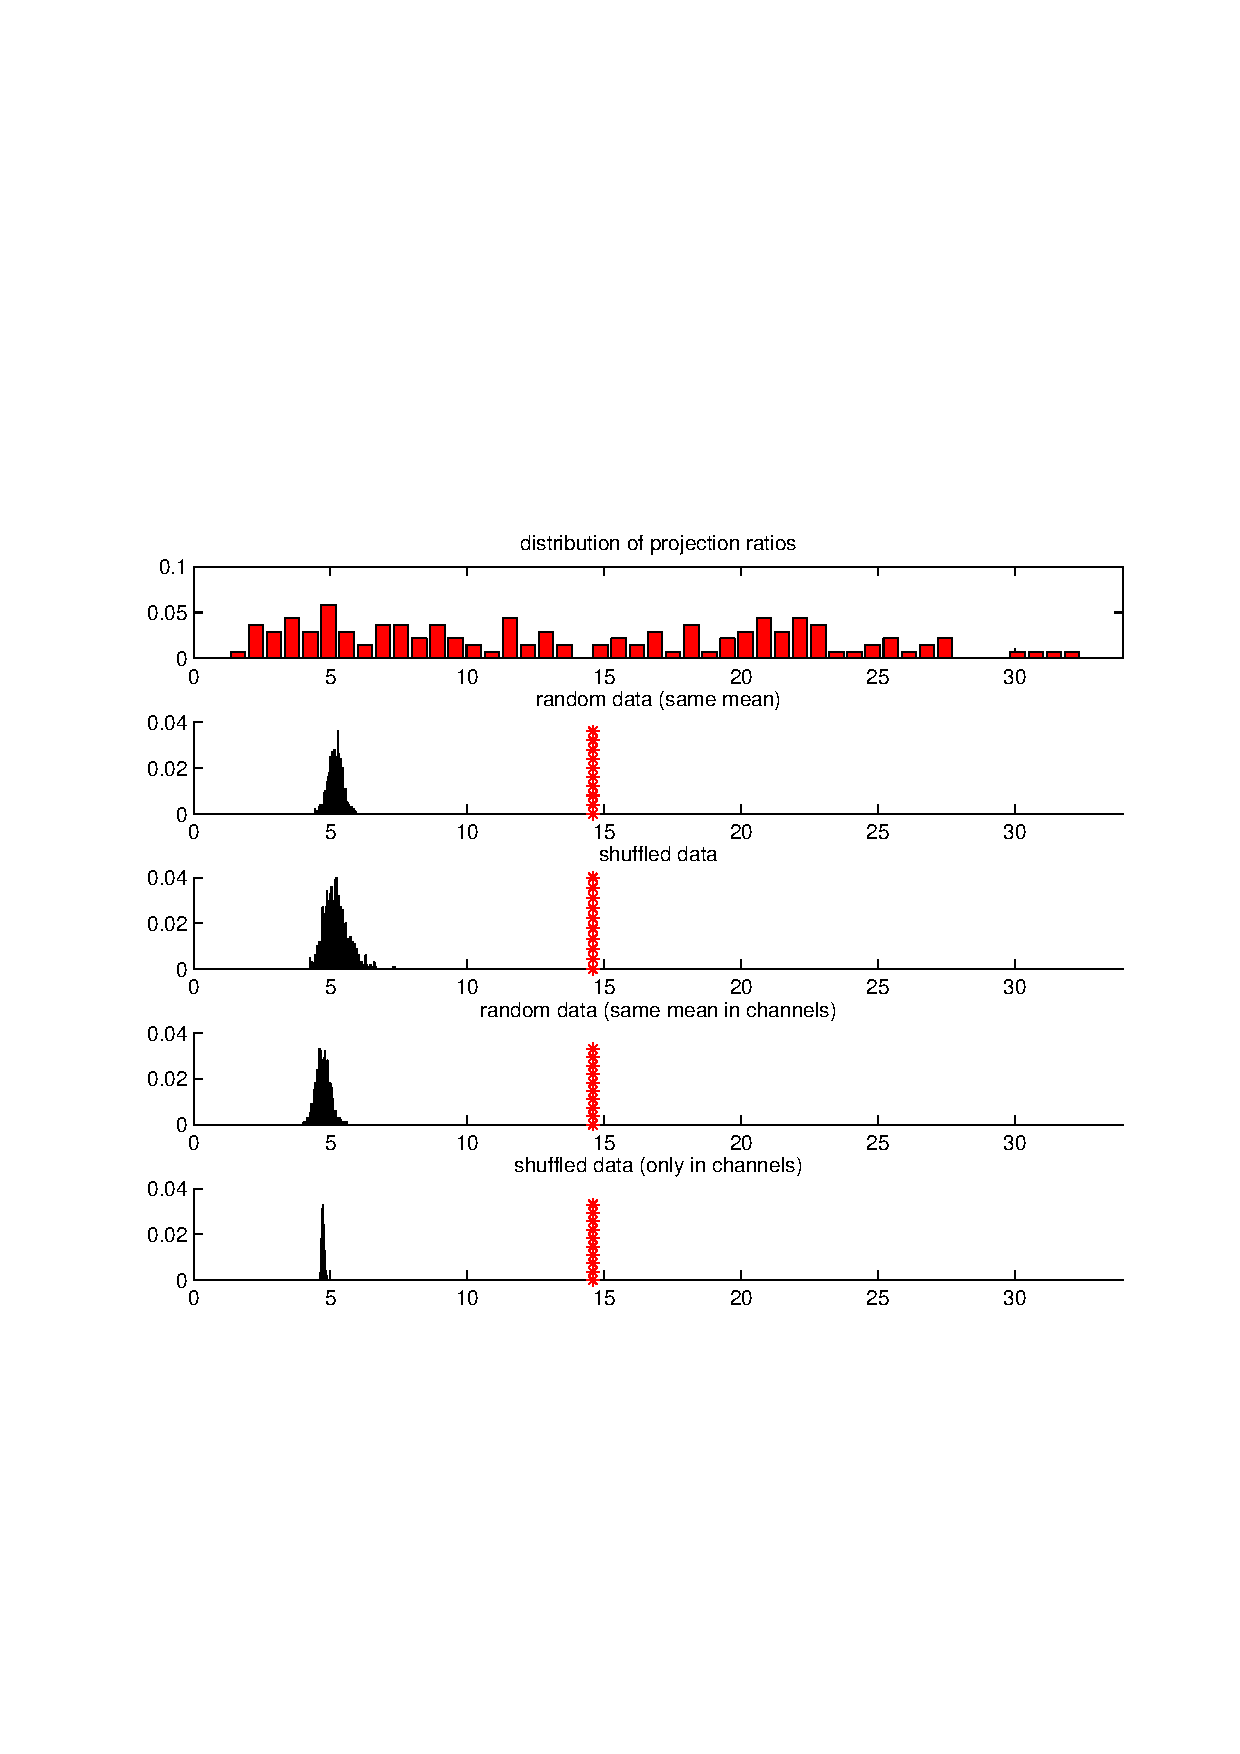
\includegraphics[width=0.8\textwidth]{images/projection_larger0_vega.pdf}
        \caption{subject V, projection analysis with sessions with 0-field sorted out}
    \label{sg:fig:images_projection_larger0_vega}
\end{figure}


% section results (end)
